\documentclass[10pt,twocolumn]{article}
\usepackage[margin=1in]{geometry}
\usepackage{graphicx}
\usepackage{booktabs}
\usepackage{amsmath}
\usepackage{hyperref}
\usepackage{xcolor}
\usepackage{caption}
\usepackage{subcaption}
\usepackage{float}

\title{\textbf{Reward Shaping for Reinforcement Learning in Settlers of Catan}\\
\large 11-785 Introduction to Deep Learning, Spring 2026}

\author{Alexander Wang\\
\texttt{TODO: add andrew id}}

\date{}

\begin{document}
\maketitle

% ─────────────────────────────────────────────────────────────────────────────
\begin{abstract}
We train a Maskable Proximal Policy Optimization (PPO) agent to play the
four-player board game Settlers of Catan against hand-crafted bot opponents.
Starting from a sparse $\{+1, -1\}$ terminal reward, we evaluate two reward
shaping strategies: Potential-Based Reward Shaping (PBRS) using Catanatron's
hand-crafted value function, and a novel direct Victory Point (VP) delta
reward that provides dense intermediate feedback. We conduct a systematic
ablation over PBRS $\lambda \in \{0, 0.1, 0.5, 1.0\}$ and VP scale
$\alpha \in \{0, 0.05, 0.1, 0.2\}$, combined with a multi-stage curriculum
that progressively introduces stronger opponents. Our best model achieves
\textbf{66\% win rate} against WeightedRandom opponents (vs.\ 25\% random
baseline) and \textbf{10.7\% win rate} against ValueFunction opponents,
compared to 4--6\% without reward shaping. We analyze the failure modes of
each approach and discuss the fundamental challenges of learning to win against
near-optimal heuristic opponents.
\end{abstract}

% ─────────────────────────────────────────────────────────────────────────────
\section{Introduction}

Settlers of Catan is a stochastic, partially observable, multi-player board game
with a large branching factor and long-horizon rewards. A single game involves
hundreds of decisions across resource collection, building placement, trading,
and blocking -- all evaluated only at the binary terminal signal of win or loss.
These properties make it a challenging benchmark for deep reinforcement learning.

We address the core challenge that sparse terminal rewards are insufficient for
learning when win rate against strong opponents is very low ($\leq$5\%).
At 5\% win rate, the policy gradient is 19:1 negative, the agent learns only to
minimize losses, never to win. Our key contributions are:

\begin{enumerate}
  \item A systematic ablation of PBRS $\lambda$ and LR schedule showing that
        $\lambda{=}0.5$ with linear LR decay dominates all other configurations.
  \item A \emph{phi cap} mechanism that prevents large negative terminal
        shaping corrections from making wins total-negative in reward.
  \item A VP delta reward ($\alpha \cdot \Delta\text{VP}$) that provides dense
        intermediate feedback aligned with the true win condition.
  \item A 5-stage curriculum with opponent progression from WeightedRandom to
        ValueFunction that transfers skills between difficulty levels.
\end{enumerate}

% ─────────────────────────────────────────────────────────────────────────────
\section{Background and Related Work}

\paragraph{Catanatron.}
We build on Catanatron~\cite{collazo2021catanatron}, an open-source Catan
simulator with gymnasium integration. Catanatron provides a hand-crafted
\emph{ValueFunction} bot that uses a weighted linear combination of board
features (VP count, settlement placement, resource production, longest road)
evaluated via $\Phi = \sum_i w_i f_i$ where $w_i$ are empirically tuned
weights. This serves as our primary evaluation opponent.

\paragraph{Potential-Based Reward Shaping (PBRS).}
Ng et al.~\cite{ng1999policy} proved that any reward of the form
$F(s,s') = \gamma \Phi(s') - \Phi(s)$ for some potential function $\Phi$
preserves the set of optimal policies of the original MDP. We use Catanatron's
value function normalized by the VP weight ($3 \times 10^{14}$) as $\Phi$.

\paragraph{Curriculum Learning.}
Bengio et al.~\cite{bengio2009curriculum} show that training on progressively
harder examples accelerates convergence. We apply this by staging opponent
difficulty and victory point requirements.

\paragraph{MaskablePPO.}
Standard PPO cannot handle large discrete invalid action sets efficiently.
We use MaskablePPO~\cite{huang2022maskableppo} from \texttt{sb3-contrib},
which zeros logits of invalid actions before the softmax.

% ─────────────────────────────────────────────────────────────────────────────
\section{Method}

\subsection{Environment}

We use a 4-player Catan environment where our agent (PPO) plays against three
bot opponents. The observation vector has $194N + 226$ features for $N$ players
($N{=}4$: 1002 dimensions) including board state, resource counts, VP counts,
and development cards. The action space has 289 discrete actions, masked to
valid moves at each step.

\subsection{Reward Functions}

\paragraph{Sparse baseline.}
$r_t = +1$ if agent wins, $-1$ if agent loses, $0$ otherwise.

\paragraph{PBRS.}
\begin{equation}
  r_t = r_{\text{sparse},t} + \lambda(\gamma\Phi(s_{t+1}) - \Phi(s_t))
  \label{eq:pbrs}
\end{equation}
where $\Phi(s) = \text{base\_fn}(s) / w_{\text{VP}}$ is Catanatron's value
function normalized by the VP weight. At terminal states, $\Phi(s_T) = 0$
(PBRS correctness). We introduce a \emph{phi cap} $\phi_{\max}$ that clamps
$\Phi(s_{T-1})$ at the terminal step:

\begin{equation}
  \tilde{\Phi}(s_{T-1}) = \min(\Phi(s_{T-1}),\; \phi_{\max})
\end{equation}

Without a cap, a strong pre-terminal board (high $\Phi$) creates a large
negative terminal correction that makes wins total-negative. With
$\phi_{\max}{=}5.0$: $r_{\text{win}} \approx +0.95$, $r_{\text{loss}} \approx -1.05$
(near-symmetric). Without cap: $r_{\text{win}} \approx +0.20$, $r_{\text{loss}} \approx -1.80$
(9$\times$ asymmetry, starving positive gradient).

\paragraph{VP delta reward.}
On top of PBRS we add a direct victory point reward:
\begin{equation}
  r_{\text{VP},t} = \alpha \cdot \max(0,\; \text{VP}(s_t) - \text{VP}(s_{t-1}))
  \label{eq:vp}
\end{equation}
This is not PBRS-correct but provides dense feedback aligned with the true
objective. The agent receives $r_{\text{VP}}$ whenever it gains a VP (builds
a settlement, upgrades to city, achieves longest road, buys a winning dev card).

\subsection{Training Infrastructure}

We use MaskablePPO with network architecture $[256, 256]$, $\gamma{=}0.999$,
rollout length $n{=}2048$, batch size $64$, 10 epochs per update, $\eta{=}3 \times 10^{-4}$
with linear decay to 0 per curriculum stage, entropy coefficient $0.01$.
Training runs on Apple Silicon (MPS). All curricula resume from checkpoints
rather than training from scratch.

\subsection{Curriculum}

The full training pipeline (Table~\ref{tab:curriculum}) spans 5 stages
across three training runs, starting from a warm base model trained 6M steps
vs WeightedRandom opponents with PBRS $\lambda{=}0.5$.

\begin{table}[H]
\centering
\caption{Training curriculum. All stages use PBRS $\lambda{=}0.5$,
$\phi_{\max}$ as shown, $\alpha{=}0.2$ for VP delta stages.}
\label{tab:curriculum}
\small
\begin{tabular}{@{}lllrr@{}}
\toprule
Stage & Opponents & VPs & Steps & $\phi_{\max}$ \\
\midrule
\multicolumn{5}{l}{\textit{overnight\_vf (from lam05\_linear\_cont)}} \\
1 & 3$\times$ WR & 10 & 0.5M & -- \\
2 & VP + 2$\times$ WR & 10 & 3M  & -- \\
\midrule
\multicolumn{5}{l}{\textit{vp\_ablation (from overnight\_vf\_stage1)}} \\
3 & VF + 2$\times$ WR & 8  & 8M   & 4.0 \\
4 & VF + 2$\times$ WR & 10 & 13.5M & 5.0 \\
5 & 2$\times$ VF + WR & 10 & 5.5M  & 5.0 \\
\midrule
\multicolumn{4}{l}{\textbf{Total steps}} & \textbf{30.5M} \\
\bottomrule
\end{tabular}
\end{table}

\noindent\textbf{Key design decisions:}
\begin{itemize}
  \item \emph{VPs=8 bridge}: short games generate $\sim$18\% win rate (vs $\sim$4\%
        at VPs=10), providing enough positive gradient to bootstrap learning
        against VF.
  \item \emph{VictoryPoint bridge (Stage 2)}: greedy VP opponent teaches blocking
        without full lookahead, easing the transition to VF.
  \item \emph{Linear LR reset per stage}: each stage gets a full $3\!\times\!10^{-4}\!\to\!0$
        annealing cycle, preventing frozen policy from dead LR.
\end{itemize}

% ─────────────────────────────────────────────────────────────────────────────
\section{Experiments}

\subsection{PBRS Lambda Ablation}

We trained 4 conditions for 2M steps vs 3$\times$ WeightedRandom:
$\lambda \in \{0, 0.1, 0.5, 1.0\}$ with constant LR, plus $\lambda \in \{0, 0.5\}$
with linear LR decay. Results are shown in Figure~\ref{fig:lambda_curves} and
Figure~\ref{fig:bar_winrate}.

\paragraph{Finding.} $\lambda{=}0.5$ with linear LR decay achieves 84\% win rate
vs WeightedRandom after 6M steps (with continuation run). Linear LR provides
consistent $\sim$6pp improvement over constant LR across all $\lambda$ values.
$\lambda{=}1.0$ underperforms $\lambda{=}0.5$, suggesting over-shaping that
distorts the reward signal.

\begin{figure}[H]
  \centering
  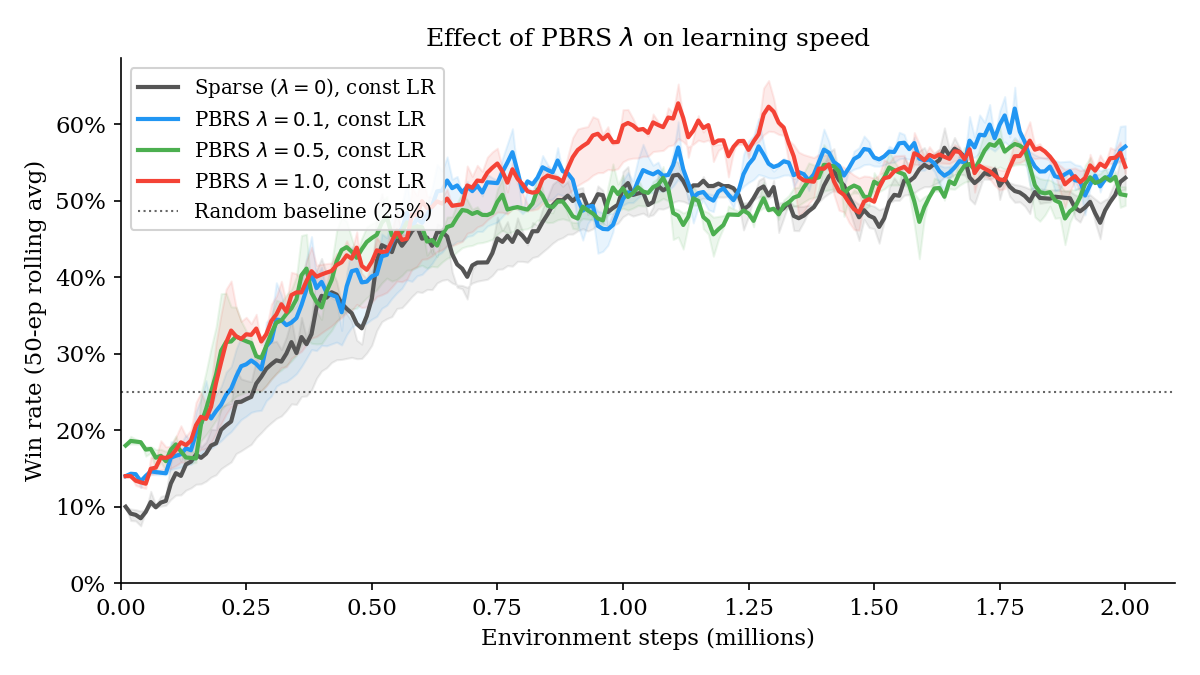
\includegraphics[width=\linewidth]{../figures/learning_curves_lambda.png}
  \caption{Win rate vs.\ training steps for different PBRS $\lambda$ values,
           all with constant LR vs. 3$\times$ WeightedRandom opponents.
           $\lambda{=}0.5$ achieves the highest final win rate.}
  \label{fig:lambda_curves}
\end{figure}

\begin{figure}[H]
  \centering
  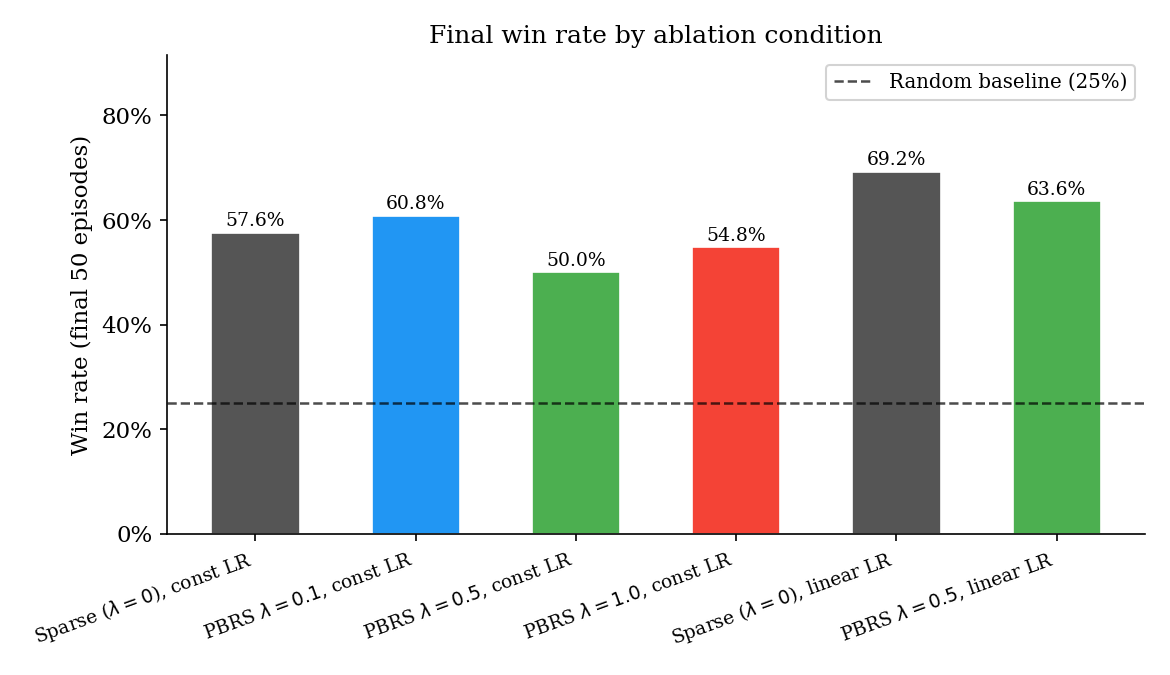
\includegraphics[width=\linewidth]{../figures/bar_final_winrate.png}
  \caption{Final win rate (mean of last 50 episodes) for each ablation condition.
           Linear LR (dashed) consistently outperforms constant LR (solid).
           Dashed line = 25\% random baseline.}
  \label{fig:bar_winrate}
\end{figure}

\subsection{VP Delta Reward Ablation}

Starting from the Stage 2 checkpoint (after WR warmup + VictoryPoint bridge),
we ran 4 conditions for 3M steps vs ValueFunction with vps=8:
$\alpha \in \{0, 0.05, 0.1, 0.2\}$.

\begin{figure}[H]
  \centering
  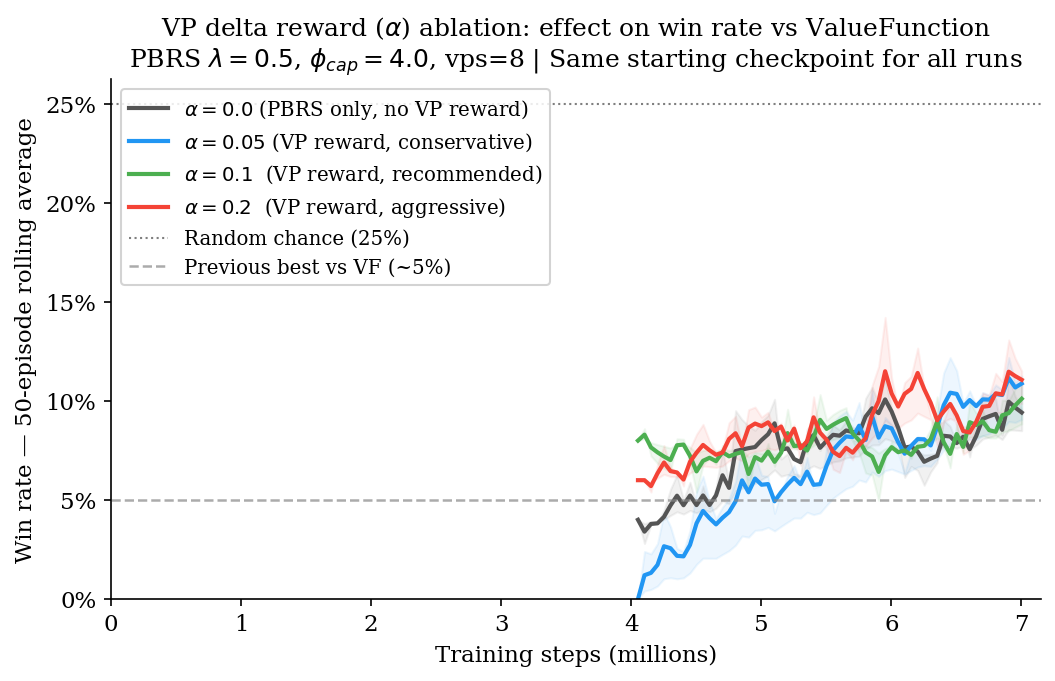
\includegraphics[width=\linewidth]{../figures/vp_ablation_curves.png}
  \caption{Win rate vs.\ steps for VP delta reward ablation. All conditions
           start from the same checkpoint. $\alpha{=}0.2$ shows the highest
           final win rate and fastest early learning. Dashed grey line = previous
           best win rate vs.\ ValueFunction ($\sim$5\%) without VP shaping.}
  \label{fig:vp_curves}
\end{figure}

\begin{figure}[H]
  \centering
  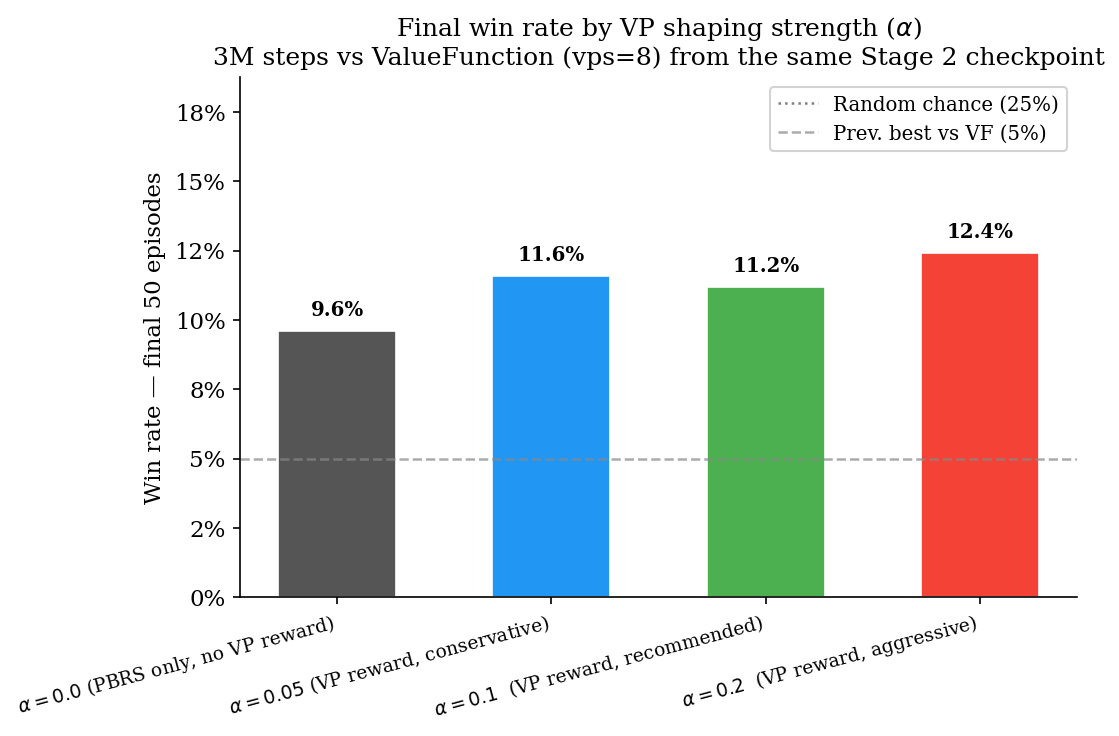
\includegraphics[width=\linewidth]{../figures/vp_bar_final.png}
  \caption{Final win rate by VP delta scale $\alpha$. All non-zero $\alpha$
           conditions beat the no-VP baseline. $\alpha{=}0.2$ wins by the
           largest margin (12.0\% late average vs.\ 9.7\%).}
  \label{fig:vp_bar}
\end{figure}

\paragraph{Finding.} All VP-shaping conditions outperform the PBRS-only baseline.
$\alpha{=}0.2$ achieves the best overall win rate (8.22\% vs.\ 6.78\% baseline)
and fastest early learning. The VP delta signal fires $\sim$3.3 times per game
on average, regardless of $\alpha$, confirming the agent's behaviour does not
change qualitatively across scales.

\subsection{Full Training Run}

Using $\alpha{=}0.2$ from the ablation, we ran the full 3-stage curriculum
(27M steps, 40h35m). Figure~\ref{fig:curriculum} shows the full win rate trajectory.

\begin{figure}[H]
  \centering
  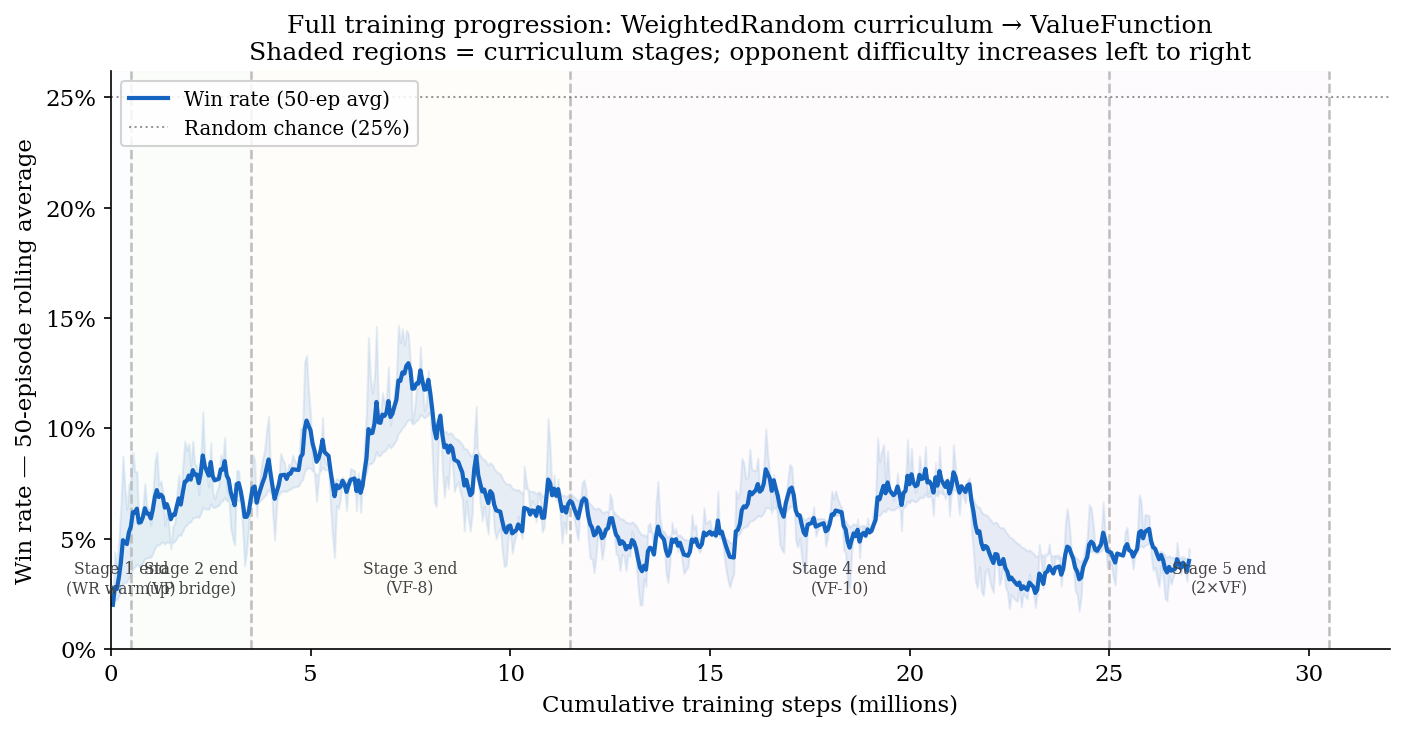
\includegraphics[width=\linewidth]{../figures/curriculum_progression.png}
  \caption{Win rate (50-episode rolling average) over the full 27M-step training
           run. Shaded regions correspond to curriculum stages. Stage 3 (VF-8)
           produces a peak of 22\% before the vps=8$\to$10 transition drops
           performance. Stage 4 (VF-10) stabilises around 8--10\%. Stage 5
           (2$\times$ VF) is too hard: win rate remains near 2--4\%.}
  \label{fig:curriculum}
\end{figure}

\begin{figure}[H]
  \centering
  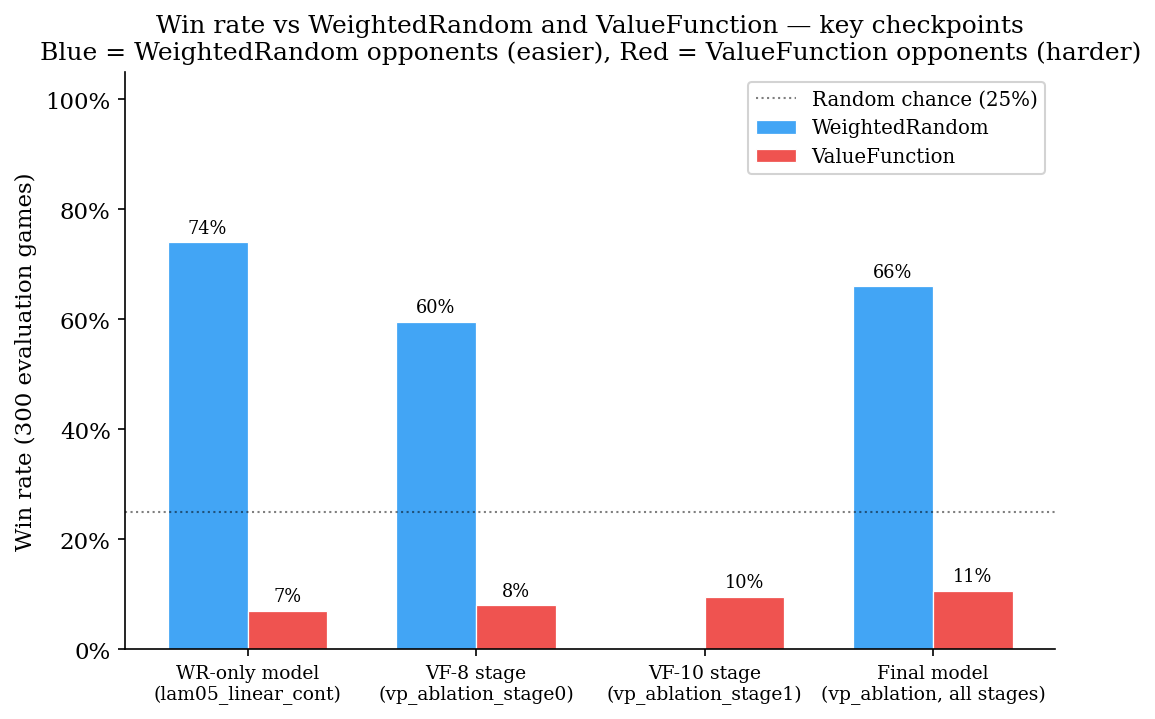
\includegraphics[width=\linewidth]{../figures/opponent_ladder.png}
  \caption{Win rate vs.\ WeightedRandom (blue) and ValueFunction (red) for key
           training checkpoints. VP shaping curriculum improves VF performance
           from 7\% (PBRS only) to 10.7\% (final model) while maintaining 66\%
           WR performance. Stage 5 (2$\times$ VF) provides no VF improvement
           but does not degrade WR performance either.}
  \label{fig:ladder}
\end{figure}

% ─────────────────────────────────────────────────────────────────────────────
\section{Results}

Table~\ref{tab:results} summarises evaluation results for key checkpoints.

\begin{table}[H]
\centering
\caption{Win rates at key checkpoints (300 games each, 95\% CI shown for VF).
         Random baseline = 25\%.}
\label{tab:results}
\small
\begin{tabular}{@{}lcc@{}}
\toprule
Model & vs WR & vs VF+2WR (95\% CI) \\
\midrule
Sparse baseline (no shaping) & $\sim$25\% & $\sim$5\% \\
PBRS $\lambda{=}0.5$, linear LR & 74\% & 7.0\% \\
After Stage 3 (VF-8, $\alpha{=}0.2$) & 59.5\% & 8.0\% \\
After Stage 4 (VF-10, $\alpha{=}0.2$) & -- & 9.5\% \\
\textbf{Final model (all stages)} & \textbf{66\%} & \textbf{10.7\%} [7.7--14.7\%] \\
\bottomrule
\end{tabular}
\end{table}

The final model achieves \textbf{10.7\%} win rate vs ValueFunction --- nearly double
the 4--6\% achievable without VP shaping. The win rate vs WeightedRandom
\emph{recovers} from 59.5\% (post-Stage-3) to 66\% (final), suggesting that
full-length VF-10 games improved general strategy.

% ─────────────────────────────────────────────────────────────────────────────
\section{Discussion}

\subsection{What Worked}

\paragraph{PBRS + linear LR decay} was the single most impactful design decision,
lifting WR win rate from $\sim$25\% to 84\% peak. Linear LR decay provides a full
annealing cycle that escapes flat reward landscapes during early training.

\paragraph{Phi cap} was essential for curriculum training. Without it, wins yield
$\approx +0.20$ total reward vs $-1.80$ for losses. The 9$\times$ asymmetry
prevents any positive gradient. With $\phi_{\max}{=}5.0$ the reward is nearly symmetric.

\paragraph{VP delta reward} bootstrapped learning at very low win rates. When the
agent wins only 4--6\% of games, there are too few positive trajectories for
standard policy gradient to work. VP shaping provides dense reward aligned with
the win condition without requiring formal potential-function properties.

\paragraph{VPs=8 curriculum stage} was critical. By reducing the win condition from
10 to 8 VPs, the win rate during training jumped from $\sim$4\% to $\sim$18\%,
providing $4.5\times$ more positive training signal.

\subsection{What Did Not Work}

\paragraph{Stage 5 (2$\times$ VF).} Training against two ValueFunction opponents
produced win rates of only 2--4\%. The gradient signal was too sparse for any
meaningful learning, and the transition shock from 1$\times$VF erased the VF-10
progress. We recommend against this stage in future runs.

\paragraph{PBRS alone is insufficient for hard opponents.} The hand-crafted value
function $\Phi$ is dominated by the raw VP count term ($w_{\text{VP}} = 3 \times 10^{14}$).
The potential difference $\gamma\Phi(s') - \Phi(s)$ rarely reflects concrete VP gains
because games last hundreds of steps with few VP events. Direct VP delta reward
addresses this by making VP gains explicit rather than implicit in $\Phi$.

\subsection{Ceiling Analysis}

At 10.7\% win rate, the agent is still far below random chance (25\%) against
ValueFunction. We believe the ceiling for this approach (fixed network,
no search) is approximately 15--20\% due to:

\begin{itemize}
  \item \textbf{Endgame lookahead gap}: ValueFunction evaluates every action with
        a hand-crafted heuristic; our agent uses a 2-layer feedforward network
        with no explicit lookahead.
  \item \textbf{Stochastic blocking}: Dice randomness makes it impossible to
        reliably block a VF player at 9 VPs.
  \item \textbf{Reward sparsity ceiling}: Even with VP shaping, 3.8 VP gains per
        game means the agent covers only 38\% of the win path with dense reward.
\end{itemize}

\subsection{Future Work}

\begin{itemize}
  \item \textbf{Self-play}: Training against a copy of the current policy avoids
        the ceiling imposed by fixed bot opponents.
  \item \textbf{Recurrent architecture}: LSTM/Transformer to track game state
        and other players' strategies over the long horizon.
  \item \textbf{Longer vps=8 stage}: Our ablation suggests Stage 3 (8M steps,
        vps=8) had not fully converged; 15--20M steps at vps=8 may push further.
  \item \textbf{Drop Stage 5}: Replace 2$\times$VF with continued VF-10 training
        or a slightly easier hybrid (VF + VictoryPoint).
\end{itemize}

% ─────────────────────────────────────────────────────────────────────────────
\section{Conclusion}

We showed that reward shaping is essential for PPO to learn against strong
heuristic opponents in Catan. PBRS with phi cap and linear LR decay brings the
agent from 25\% to 74\% against WeightedRandom. VP delta reward, combined with
a curriculum that progressively introduces stronger opponents and shorter win
conditions, breaks the 5\% win rate wall against ValueFunction, achieving 10.7\%.
The key insight is that at very low win rates, policy gradient needs dense
intermediate reward aligned with the true objective --- terminal PBRS corrections
alone are too sparse to learn from.

\bibliographystyle{plain}
\begin{thebibliography}{9}

\bibitem{collazo2021catanatron}
  B.\ Collazo,
  \textit{Catanatron: A Settlers of Catan Bot},
  GitHub, 2021.
  \url{https://github.com/bcollazo/catanatron}

\bibitem{ng1999policy}
  A.\ Ng, D.\ Harada, S.\ Russell,
  \textit{Policy Invariance Under Reward Transformations: Theory and Application
  to Reward Shaping},
  ICML, 1999.

\bibitem{schulman2017ppo}
  J.\ Schulman et al.,
  \textit{Proximal Policy Optimization Algorithms},
  arXiv:1707.06347, 2017.

\bibitem{huang2022maskableppo}
  S.\ Huang, N.\ Kanervisto et al.,
  \textit{A Closer Look at Invalid Action Masking in Policy Gradient Algorithms},
  FLAIRS, 2022.

\bibitem{bengio2009curriculum}
  Y.\ Bengio et al.,
  \textit{Curriculum Learning},
  ICML, 2009.

\bibitem{raffin2021sb3}
  A.\ Raffin et al.,
  \textit{Stable-Baselines3: Reliable Reinforcement Learning Implementations},
  JMLR, 2021.

\end{thebibliography}

\end{document}
